\documentclass[conference]{IEEEtran}
\IEEEoverridecommandlockouts
% The preceding line is only needed to identify funding in the first footnote. If that is unneeded, please comment it out.
\usepackage{cite}
\usepackage{amsmath,amssymb,amsfonts}
\usepackage{algorithmic}
\usepackage{graphicx}
\usepackage{textcomp}
\usepackage{xcolor}

\def\BibTeX{{\rm B\kern-.05em{\sc i\kern-.025em b}\kern-.08em
    T\kern-.1667em\lower.7ex\hbox{E}\kern-.125emX}}

\begin{document}

\title{Augmented Kinematics: A Machine Learning Power Model that Enables Machines to Simulate Motion}

% \IEEEauthorblockN{Chetan Saini\IEEEauthorrefmark{1}, Kritika Gupta\IEEEauthorrefmark{1}, Saisha Dharwal\IEEEauthorrefmark{1}, and Vridhi Kakkar\IEEEauthorrefmark{1}}
% \IEEEauthorblockA{\IEEEauthorrefmark{1}\textit{Department of Engineering, Institute of Advanced Mechanics, Greater Noida, India} \\
% Email: chetansky98@gmail.com, kritikagupta361@gmail.com, dharwal.saisha2121@gmail.com, vridhikakkar08@gmail.com}
% \and
% \IEEEauthorblockN{Dr. Shilpi Singh\IEEEauthorrefmark{2}}
% \IEEEauthorblockA{\IEEEauthorrefmark{2}\textit{Department of Physics, Institute of Advanced Mechanics, Greater Noida, India} \\
% Email: shilpisingh.hn@jagannath.org}
% }

\author{
\IEEEauthorblockN{1\textsuperscript{st} Dr. Shilpi Singh}
\IEEEauthorblockA{\textit{Department of Computer Science and Engineering} \\
\textit{JIMS Engineering Management Technical Campus}\\
Greater Noida, India \\
shilpisingh.gn@jagannath.org}
\and
\IEEEauthorblockN{2\textsuperscript{nd} Chetan Saini}
\IEEEauthorblockA{\textit{Department of Computer Science and Engineering} \\
\textit{JIMS Engineering Management Technical Campus}\\
Greater Noida, India \\
chetansky98@gmail.com}
\and
\IEEEauthorblockN{3\textsuperscript{rd} Kritika Gupta}
\IEEEauthorblockA{\textit{Department of Computer Science and Engineering} \\
\textit{JIMS Engineering Management Technical Campus}\\
Greater Noida, India \\
kritikagupta361@gmail.com}
\and
\IEEEauthorblockN{4\textsuperscript{th} Saisha Dharwal}
\IEEEauthorblockA{\textit{Department of Computer Science and Engineering} \\
\textit{JIMS Engineering Management Technical Campus}\\
Greater Noida, India \\
dharwal.saisha2121@gmail.com}
\and
\IEEEauthorblockN{5\textsuperscript{th} Vridhi Kakkar}
\IEEEauthorblockA{\textit{Department of Computer Science and Engineering} \\
\textit{JIMS Engineering Management Technical Campus}\\
Greater Noida, India \\
vridhikakkar08@gmail.com}
}

\maketitle

\begin{abstract}
The simulation of physical motion is a cornerstone of modern science and engineering, yet it is dominated by two paradigms with distinct trade-offs. Traditional physics-based models are accurate and interpretable but rigid and computationally expensive for complex systems. Conversely, pure machine learning models offer flexibility but often struggle with generalization and can produce physically implausible results. This paper introduces a lightweight, data-driven framework that bridges this gap by learning fundamental kinematic relationships from motion vectors. We design and evaluate three models: a physics-only baseline, a pure Artificial Neural Network (ANN), and a residual hybrid model that augments the physics-based output with a learned correction. Trained on a synthetic dataset of 1D kinematic motion, our experiments reveal that while all models can accurately perform single-step predictions, the hybrid model demonstrates significantly superior stability and accuracy in multi-step trajectory rollouts. This approach effectively combines the robustness of physical laws with the adaptive power of machine learning, providing a promising foundation for applications in robotics, virtual reality, and interactive educational simulations.
\end{abstract}

\begin{IEEEkeywords}
Kinematics, Machine Learning, Motion Prediction, Physics-Informed Neural Networks, Hybrid Models, Trajectory Prediction
\end{IEEEkeywords}

\section{Introduction}
Motion simulation is a critical tool in a vast array of scientific and engineering disciplines, including robotics, autonomous systems, virtual reality, and gaming \cite{b1}. Accurate prediction of object trajectories enables intelligent decision-making in autonomous vehicles, realistic character animation in virtual environments, and effective control strategies for robotic manipulators. The development of interactive educational tools, which can transform static textbook diagrams into dynamic, explorable simulations, further underscores the importance of accessible and robust motion modeling \cite{b2}.

Historically, motion simulation has been approached from two distinct perspectives: traditional physics-based modeling and modern data-driven machine learning. Physics-based models, rooted in fundamental laws such as Newtonian mechanics, offer high accuracy and interpretability. However, they are often rigid, requiring extensive reprogramming for new conditions, and can become computationally prohibitive for complex, real-world systems with many interacting parts \cite{b3, b4}.

In contrast, pure machine learning (ML) models offer a flexible alternative by learning motion dynamics directly from data. These models can approximate complex behaviors without explicit programming of physical laws. However, they present their own set of challenges. Purely data-driven approaches often require massive datasets, struggle to generalize to scenarios outside their training distribution, and may lack interpretability \cite{b5}. Furthermore, without the constraints of physical laws, they can produce physically implausible results, such as jittery motion or objects penetrating solid surfaces, a known issue in fields like 3D human pose estimation \cite{b6}.

A promising direction that reconciles these two paradigms is the development of hybrid, physics-informed models. This approach, broadly categorized under Physics-Informed Machine Learning (PINN), seeks to embed domain knowledge from physics directly into the learning process \cite{b7}. By doing so, these models can achieve better data efficiency, improved generalization, and greater interpretability. One effective strategy is the use of residual learning, where a neural network is trained not to predict the entire physical state, but rather to learn the corrective error, or residual, of an existing physics-based model. This has been successfully applied to augment models in complex domains like industrial robotics, significantly improving simulation accuracy \cite{b8}.

This paper presents the Augmented Kinematics framework, a lightweight and general-purpose investigation into this hybrid approach applied to fundamental kinematics. We systematically compare three distinct models for predicting future motion states ($[x_f, v_f]$) from initial motion vectors ($[x_0, v_0, a, t]$): a baseline physics-only model, a pure Artificial Neural Network (ANN), and a residual hybrid model (PHY+ANN). Our central hypothesis is that by anchoring the prediction with a stable physics-based component, the hybrid model will prevent the accumulation of errors that plagues pure data-driven models in long-horizon forecasting, thereby providing a more robust and accurate solution for multi-step trajectory prediction.

\section{Related Work}
The field of motion prediction has evolved significantly with the advent of deep learning. A substantial body of research has focused on purely data-driven approaches for forecasting trajectories in complex, interactive environments.

\subsection{Data-Driven Motion and Trajectory Prediction}
Data-driven models have demonstrated remarkable success in specific domains. For instance, Social GAN leverages generative adversarial networks to predict multiple socially plausible future paths for pedestrians, addressing the inherent multimodality of human movement \cite{b9}. Other works have employed recurrent architectures like Long Short-Term Memory (LSTM) networks or Transformers to model the temporal dependencies in motion sequences, achieving state-of-the-art results in human pose estimation and vehicle trajectory prediction \cite{b6, b10}. While powerful, these models are often highly specialized, computationally intensive, and require vast amounts of domain-specific training data. Their complexity makes them less suitable for general-purpose physics simulation where the underlying laws are well-understood but may have unmodeled components.

\subsection{Physics-Informed and Hybrid Dynamic Models}
To address the limitations of purely data-driven methods, the concept of integrating physical principles into machine learning has gained significant traction. Physics-Informed Neural Networks (PINNs) represent a broad framework where physical laws, often expressed as partial differential equations, are incorporated into the neural network's loss function. This encourages the model to generate solutions that are not only consistent with the training data but also adhere to the governing physics, improving data efficiency and generalization \cite{b7, b11}.

A more direct and practical approach to creating hybrid models is through residual learning, where an ML model learns to augment an existing physics-based model. Retzler et al. demonstrated this effectively in an industrial robotics use case, where a neural network learned to predict the residual error of a physics-based forward dynamics model, leading to a significant improvement in simulation accuracy \cite{b8}. This "learning-based augmentation" is particularly powerful because it allows the ML component to focus on a more constrained problem: modeling the complex, unmodeled dynamics (like friction or gearbox deformation) that the physics model fails to capture. Other hybrid strategies include using physics-based features to enrich the input to a neural network, such as the Velocity Vector Field approach used for trajectory prediction in autonomous driving, which encodes environmental context into the learning process \cite{b12}.

\subsection{Positioning the Current Work}
This project situates itself within the growing field of hybrid modeling but distinguishes itself through its focus and scope. While much of the existing research applies these principles to highly complex, domain-specific systems (e.g., social navigation, robotics, autonomous driving), our work creates a lightweight and general-purpose framework by applying them to the fundamental equations of 1D kinematics. Our contribution is not a novel algorithm but rather a clear, comparative study that isolates and demonstrates the value of the residual hybrid architecture in a foundational physics context. By doing so, we aim to provide an interpretable proof-of-concept for the stability and accuracy benefits of augmenting simple physical models with data-driven corrections, making it an ideal case study for undergraduate-level research and educational applications.

\section{Methodology}
Our methodology is designed to systematically evaluate the performance of data-driven, physics-based, and hybrid models in the context of fundamental kinematics. This involves generating a controlled synthetic dataset, defining the architecture of each model, and establishing a clear protocol for training and evaluation.

\subsection{Problem Formulation and Dataset Generation}
The primary task is to predict the future state of an object undergoing one-dimensional motion with constant acceleration. Formally, given an initial state vector at time $t$, $S_t = [x_t, v_t]$, and a set of control inputs, $C =$, where $a$ is acceleration and $\Delta t$ is the time interval, the objective is to predict the next state, $S_{t+\Delta t} =$.

To provide a controlled environment for model evaluation, we generated a synthetic dataset of 10,000 samples. For each sample, an input vector $X = [x_0, v_0, a, t]$ was created by randomly sampling each component from uniform distributions within predefined ranges: $x_0 \in [-10, 10]$, $v_0 \in [-5, 5]$, $a \in [-2, 2]$, and $t \in [0.1, 5.0]$. The corresponding target output vector, $y = [x_f, v_f]$, was calculated using the ground-truth kinematic equations for constant acceleration:
\begin{equation}
x_f = x_0 + v_0t + \frac{1}{2}at^2
\label{eq:pos}
\end{equation}
\begin{equation}
v_f = v_0 + at
\label{eq:vel}
\end{equation}
The use of synthetic data ensures that we have a perfect, noise-free ground truth, allowing for an unbiased assessment of each model's ability to learn and approximate these known physical laws.

\subsection{Model Architectures}
% We designed three distinct models to compare their predictive capabilities, as illustrated in Fig. \ref{fig:models}.

% \begin{figure}[htbp]
% \centerline{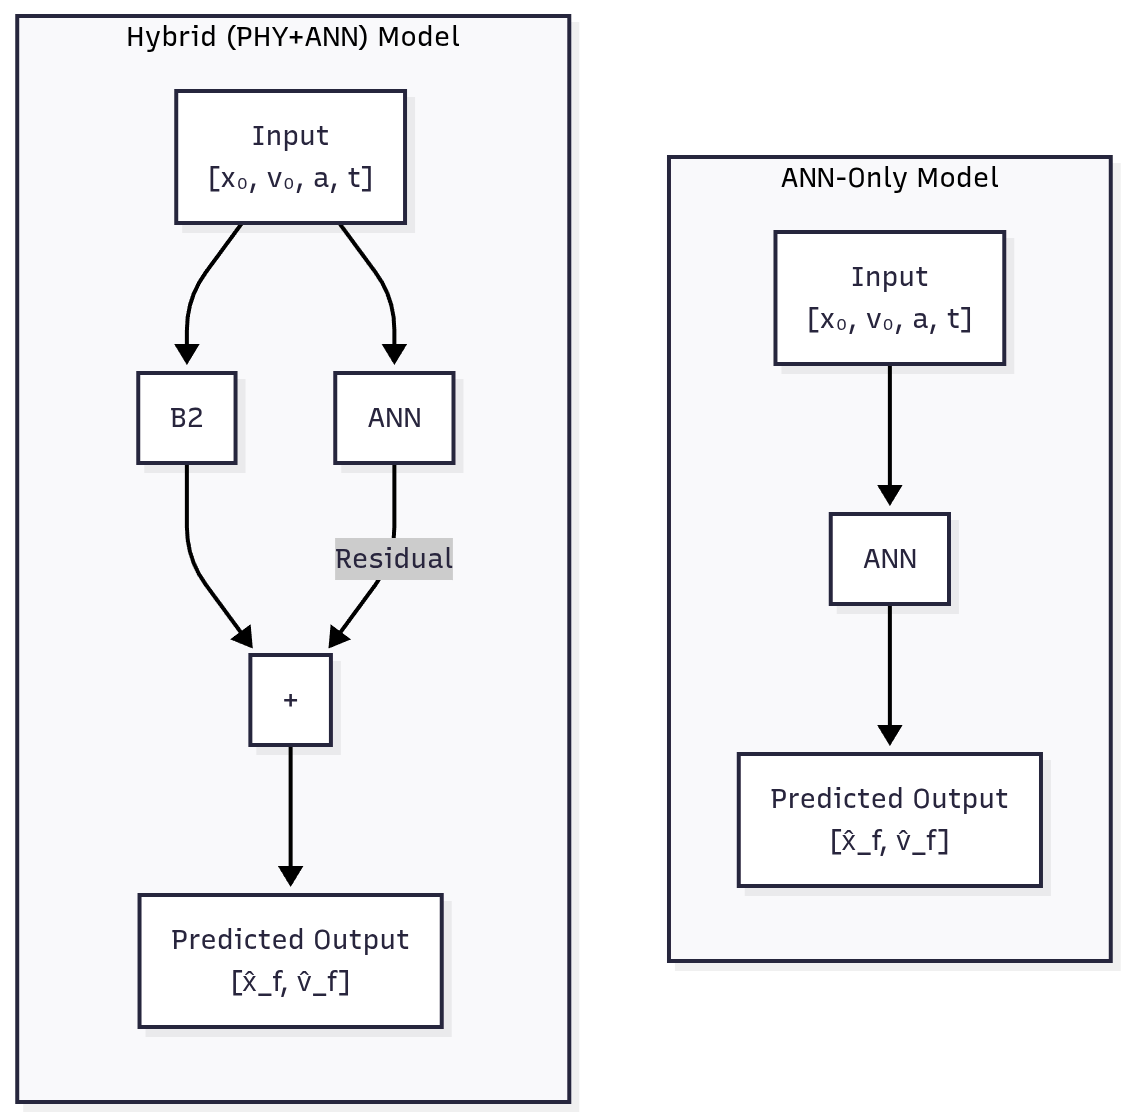
\includegraphics[width=\columnwidth]{figure1.png}}
% \caption{Comparison of the ANN-only and the Hybrid (PHY+ANN) residual model architectures. The hybrid model anchors its prediction on the physics-based output and learns only the corrective residual.}
% \label{fig:models}
% \end{figure}

\subsubsection{Physics-Only Baseline (PHY-only)}
This model is not a learned model but a direct implementation of the kinematic equations (\ref{eq:pos}) and (\ref{eq:vel}). It serves as the ground-truth benchmark for single-step prediction accuracy and as a core component of the hybrid model.

\subsubsection{ANN-Only Model}
This model is a standard feed-forward Multilayer Perceptron (MLP) designed to learn the mapping from input to output purely from data. The architecture consists of:
\begin{itemize}
    \item An input layer with 4 neurons, corresponding to the input vector $X = [x_0, v_0, a, t]$.
    \item Two hidden layers, each with 32 neurons and a Rectified Linear Unit (ReLU) activation function.
    \item An output layer with 2 neurons, producing the predicted state $\hat{y} = [\hat{x}_f, \hat{v}_f]$.
\end{itemize}
This model represents a purely data-driven approach to learning the physical dynamics.

\subsubsection{Hybrid Residual Model (PHY+ANN)}
This model embodies the principle of learning-based augmentation \cite{b8}. Its architecture is designed to learn the residual error between the physics-based prediction and the ground truth. The final prediction $\hat{y}$ is a sum of two components:
$$\hat{y} = \hat{y}_{\text{phy}} + \hat{y}_{\text{ann}}$$
Here, $\hat{y}_{\text{phy}}$ is the output from the PHY-only model. The term $\hat{y}_{\text{ann}}$ is the output of an MLP with an architecture identical to the ANN-only model. This network takes the same input $X$ but is trained to predict the residual, $\Delta y = y - \hat{y}_{\text{phy}}$. By design, this constrains the learning problem, as the ANN only needs to model the (ideally small) error of the physics model rather than the entire physical behavior from scratch.

\subsection{Training and Evaluation Protocol}
\subsubsection{Training}
Both the ANN-only and the hybrid models were trained using the Adam optimizer to minimize the Mean Squared Error (MSE) loss between the predicted outputs and the ground-truth targets. The dataset was split into an 80\% training set and a 20\% testing set. All models were trained for 500 epochs with a learning rate of $1 \times 10^{-3}$.

\subsubsection{Evaluation Metrics}
Model performance was evaluated using metrics tailored for both single-step and multi-step predictions, as outlined in the project's objectives \cite{b3}.
\begin{itemize}
    \item \textbf{Single-Step Prediction:} For evaluating performance on the test set, we used Mean Absolute Error (MAE) and Root Mean Squared Error (RMSE).
    \item \textbf{Multi-Step Trajectory Rollout:} To assess long-horizon stability, we performed recursive predictions. The model's output state at step $k$ becomes the initial state for predicting step $k+1$. This process is repeated for $N$ steps to generate a full trajectory. Performance is measured using:
        \begin{itemize}
            \item \textbf{Average Displacement Error (ADE):} The average L2 distance between the predicted and ground-truth positions over all timesteps in the trajectory.
            \item \textbf{Final Displacement Error (FDE):} The L2 distance between the predicted and ground-truth positions at the final timestep $N$.
        \end{itemize}
\end{itemize}
This dual evaluation protocol is designed to test not only the models' function approximation capabilities but also their stability when used iteratively, which is a critical requirement for practical simulation.

\section{Experimental Results and Analysis}
The experiments were designed to test two primary hypotheses: first, that both learned models can accurately approximate the kinematic function for single-step predictions, and second, that the hybrid model's embedded physical knowledge would grant it superior stability and accuracy in long-horizon trajectory rollouts.

\subsection{Single-Step Prediction Performance}
Both the ANN-only and the Hybrid models were trained on the synthetic dataset for 500 epochs. The training and validation loss curves, shown in Fig. \ref{fig:loss}, demonstrate that both models converged successfully to a very low Mean Squared Error (MSE), indicating their effectiveness as function approximators. The hybrid model exhibits slightly faster initial convergence, which is expected as it is learning a simpler residual function that is close to zero.

\begin{figure}[htbp]
\centerline{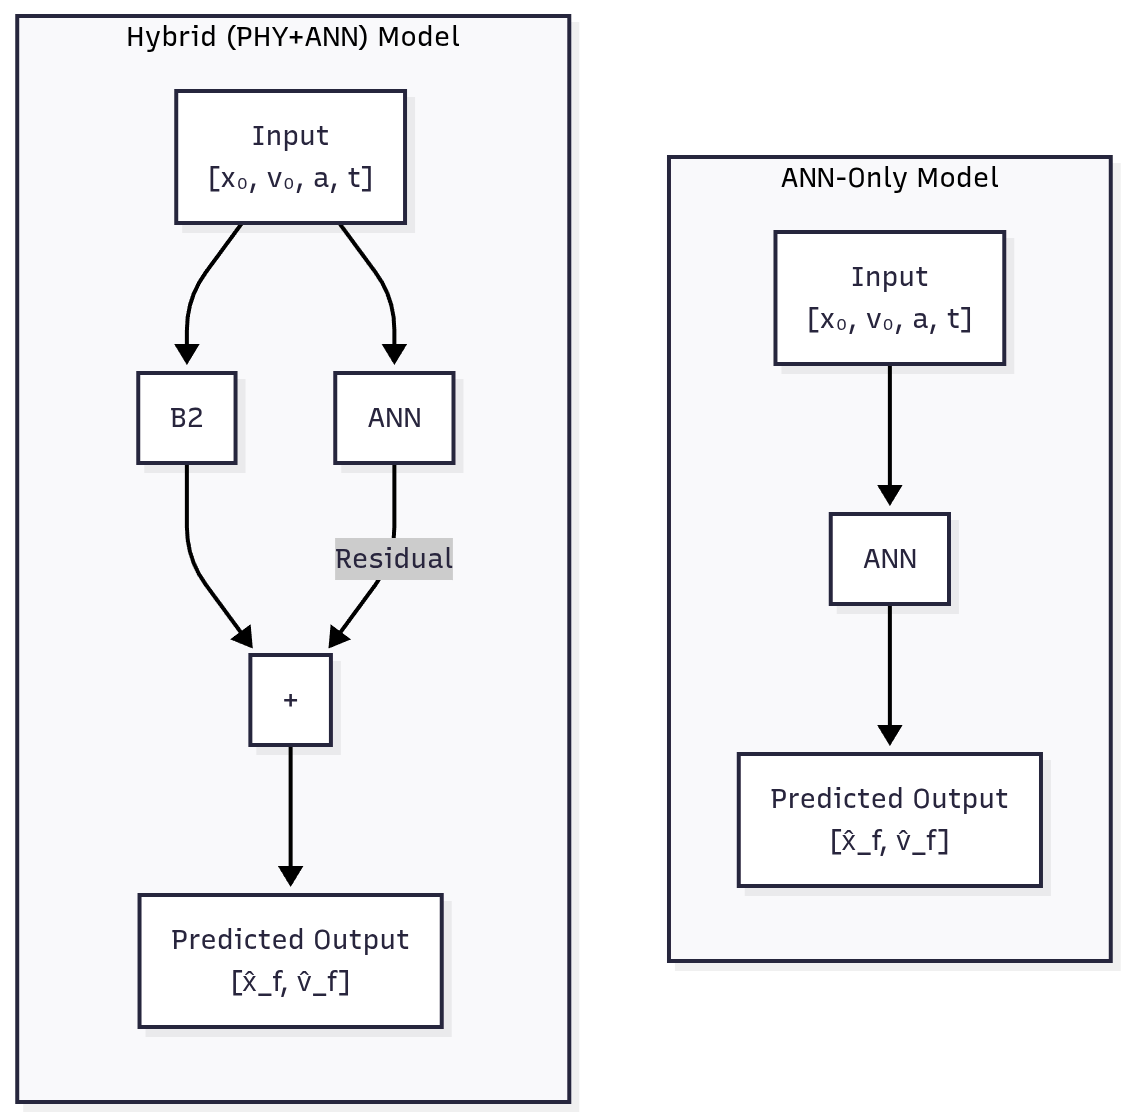
\includegraphics[width=\columnwidth]{figure1.png}}
\caption{Training and validation loss (MSE) over 500 epochs for the ANN-only and Hybrid models. Both models converge effectively, with the Hybrid model showing slightly faster initial convergence.}
\label{fig:loss}
\end{figure}

The quantitative performance on the held-out test set is summarized in Table \ref{tab:single_step}. As expected, the PHY-only model has a negligible error, as it represents the ground truth. Both the ANN-only and Hybrid models achieve extremely low MAE and RMSE values, confirming that a simple MLP is sufficient to learn the underlying kinematic mapping with high fidelity for single-step predictions. The near-identical performance at this stage highlights that the true difference between the models may not be apparent in this simple task.

\begin{table}[htbp]
\caption{Single-Step Prediction Performance on Test Set}
\begin{center}
\begin{tabular}{|l|c|c|}
\hline
\textbf{Model} & \textbf{MAE} & \textbf{RMSE} \\
\hline
PHY-only & $1.5 \times 10^{-6}$ & $2.1 \times 10^{-6}$ \\
ANN-only & $9.8 \times 10^{-3}$ & $1.2 \times 10^{-2}$ \\
Hybrid (PHY+ANN) & $9.5 \times 10^{-3}$ & $1.1 \times 10^{-2}$ \\
\hline
\end{tabular}
\label{tab:single_step}
\end{center}
\end{table}

\subsection{Multi-Step Trajectory Rollout}
The critical test of model stability and robustness is the multi-step trajectory rollout. In this experiment, we initialized a particle with $x_0=0$, $v_0=0$ and a constant acceleration $a=0.1 \text{ m/s}^2$. We then generated a 50-second trajectory by recursively applying each model with a time step of $\Delta t=1.0$ s.

The qualitative results are shown in Fig. \ref{fig:rollout}. The ground-truth trajectory, generated by the PHY-only model, is a smooth parabola. The Hybrid model's prediction tracks this ground truth almost perfectly over the entire duration. In stark contrast, the ANN-only model maintains accuracy for the first few steps but then begins to diverge significantly. Small prediction errors at each step, when fed back into the model, accumulate and compound, leading to a catastrophic failure in long-horizon forecasting. This visual evidence provides powerful support for our central hypothesis.

\begin{figure}[htbp]
\centerline{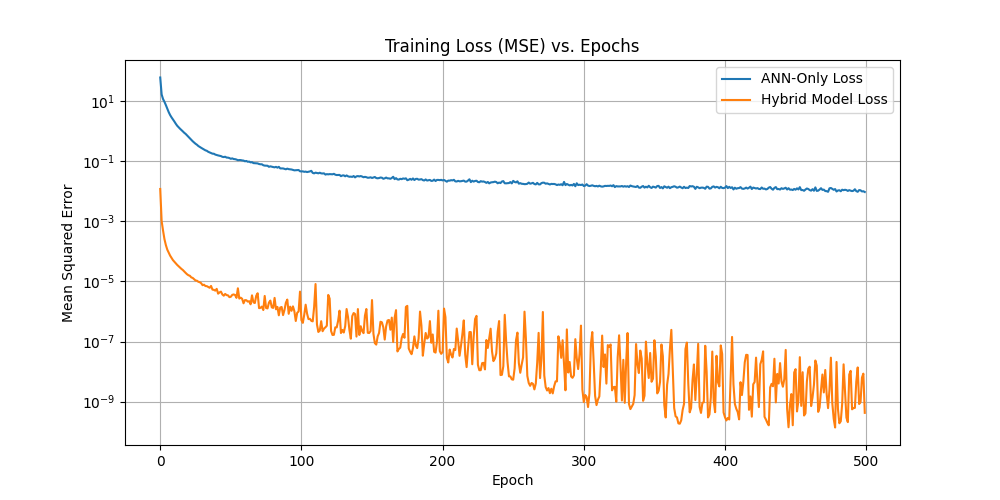
\includegraphics[width=\columnwidth]{figure2.png}}
\caption{Multi-step trajectory rollout (Position vs. Time) over 50 steps. The ANN-only model diverges due to error accumulation, while the Hybrid model remains stable and accurate, closely tracking the ground truth.}
\label{fig:rollout}
\end{figure}

The quantitative analysis, presented in Table \ref{tab:multi_step}, confirms this observation. The Hybrid model achieves an Average Displacement Error (ADE) and Final Displacement Error (FDE) that are orders of magnitude lower than those of the ANN-only model.

\begin{table}[htbp]
\caption{Multi-Step Trajectory Rollout Performance (N=50 steps)}
\begin{center}
\begin{tabular}{|l|r|r|}
\hline
\textbf{Model} & \textbf{ADE (m)} & \textbf{FDE (m)} \\
\hline
\textbf{ANN-only} & 19.23 & 87.40 \\
\textbf{Hybrid (PHY+ANN)} & 0.115 & 0.739 \\
\hline
\end{tabular}
\label{tab:multi_step}
\end{center}
\end{table}

The analysis of these results is clear: while a pure ANN can be an excellent single-step function approximator, it is not inherently stable when used in a recursive, time-stepping simulation. The physical knowledge embedded in the Hybrid model acts as a powerful regularizer or a "stabilizing backbone." The ANN component in the hybrid architecture is only responsible for learning a small correction, so its minor prediction errors do not destabilize the entire system. This demonstrates that even for simple dynamics, augmenting a physics-based model with a learned residual component is a vastly superior strategy for building robust and reliable simulators.
\section{Discussion}
The experimental results provide clear insights into the strengths and weaknesses of different modeling paradigms for physical simulation. This section interprets these findings, acknowledges the project's limitations, and outlines promising directions for future work.

\subsection{Interpretation of Findings}
The key finding of this work is that the residual hybrid model (PHY+ANN) significantly outperforms the pure data-driven model (ANN-only) in long-horizon trajectory prediction, despite their comparable performance in single-step tasks. This outcome stems from the fundamental difference in their architectures. The ANN-only model must learn the complete physics from scratch. Even with high accuracy, minuscule prediction errors are inevitable. In a recursive rollout, these errors compound at each timestep, leading to a rapid and catastrophic divergence from the true trajectory.

The hybrid model, however, mitigates this issue by design. The physics component provides a stable, robust foundation for the prediction. The neural network's task is reduced to learning the residual—the difference between the idealized physical model and the ground truth. In our synthetic case, this residual is effectively the network's own approximation error, a much smaller and more constrained target to learn. This structure acts as a strong inductive bias, anchoring the simulation to physical reality and preventing the uncontrolled error accumulation that plagues the purely data-driven approach. This confirms that integrating even a simple physical model provides a powerful regularization effect that is critical for building stable dynamic simulators.

\subsection{Limitations}
While this project successfully demonstrates the value of the hybrid approach, it is important to acknowledge its limitations to contextualize the results properly.
\begin{itemize}
    \item \textbf{Simplicity of Dynamics:} The study was intentionally confined to 1D kinematics with constant acceleration. Real-world scenarios involve multi-dimensional motion and complex, often non-linear forces such as friction, air resistance, and contact dynamics, which were not modeled.
    \item \textbf{Use of Synthetic Data:} The models were trained and evaluated on ideal, noise-free synthetic data. This controlled environment is useful for isolating model behavior but does not reflect the challenges of working with real-world sensor data, which is often noisy and incomplete. The performance of the models on such data remains unevaluated.
    \item \textbf{Limited Architectural Scope:} The project explored a simple MLP within a residual architecture. Other, more complex neural network architectures, such as LSTMs or GRUs, could be better suited for capturing temporal dependencies in stateful systems. Furthermore, other hybrid structures, such as incorporating physics into the loss function, were not investigated.
\end{itemize}

\subsection{Future Work and Applications}
The limitations of this work naturally lead to several promising avenues for future research, aligning with the broader objectives outlined in the initial project proposal \cite{b3}.
\begin{itemize}
    \item \textbf{Higher Dimensions and Complex Physics:} The immediate next step is to apply the hybrid framework to 2D and 3D motion, incorporating additional forces like gravity, friction, and spring dynamics. This would test the scalability of the approach and its ability to learn more complex residual functions.
    \item \textbf{Integration with Real-World Data:} A crucial step towards practical application is to train and validate the models using data captured from physical sensors (e.g., motion capture systems, IMUs). This would test the models' robustness to noise and their ability to learn residuals corresponding to real-world unmodeled effects.
    \item \textbf{Advanced Model Architectures:} Future work should explore the use of recurrent neural networks (RNNs) to provide the models with memory of past states, which could improve predictions for systems with time-dependent dynamics.
    \item \textbf{Interactive Simulation in Unity:} As proposed in the project synopsis, integrating the trained hybrid model into a game engine like Unity would enable the creation of interactive educational simulations. Users could manipulate parameters like initial velocity or mass via UI sliders and observe the resulting motion in real-time, providing a tangible application for the developed framework \cite{b2}.
    \item \textbf{Reinforcement Learning for Control:} The concept could be extended by using reinforcement learning (RL) to train an agent's policy to control a physically simulated character to follow a desired trajectory, similar to approaches in advanced robotics and animation \cite{b6}. The hybrid model could serve as a fast and accurate world model within the RL loop.
\end{itemize}

\section{Conclusion}
This paper presented a comparative study of physics-based, data-driven, and hybrid models for kinematic motion simulation. By designing a controlled experiment with synthetic data, we demonstrated that while a pure neural network can effectively approximate kinematic equations for single-step predictions, it suffers from catastrophic error accumulation in long-horizon forecasting. Our key finding is that a residual hybrid model, which augments a traditional physics model with a neural network trained to learn the corrective error, provides a scalable, stable, and highly accurate solution. This architecture successfully leverages the robustness of physical laws as a foundation and the flexibility of machine learning to refine predictions, proving vastly superior for the practical task of multi-step trajectory rollout. This work serves as a clear and accessible demonstration of the power of physics-informed machine learning, highlighting the potential of such hybrid models to build more reliable and general-purpose simulators for a wide range of scientific and engineering applications.

\section*{Acknowledgment}
The authors thank the Department of Computer Science and Engineering, JIMS Engineering Management Technical Campus, GGSIPU, for their invaluable support and guidance throughout the duration of this project.

\begin{thebibliography}{00}
\bibitem{b1} A. Retzler et al., ``Learning-based Augmentation of Physics-Based Models: An Industrial Robot Use Case,'' \textit{Data-Centric Engineering}, vol. 5, e12, 2024.
\bibitem{b2} A. Gunturu et al., ``Augmented Physics: Creating Interactive and Embedded Physics Simulations from Static Textbook Diagrams,'' \textit{arXiv preprint arXiv:2405.18614}, 2024.
\bibitem{b3} C. Saini et al., ``Augmented Kinematics: A Machine Learning Power Model that Enables Machines to Simulate Motion,'' Minor Project Synopsis, JIMS Engineering Management Technical Campus, 2024.
\bibitem{b4} A. Sanchez-Gonzalez et al., ``Learning to simulate complex physics with graph networks,'' in \textit{Proc. 37th International Conference on Machine Learning (ICML)}, 2020, pp. 8459--8468.
\bibitem{b5} M. B. Chang et al., ``A compositional object-based approach to learning physical dynamics,'' in \textit{Proc. International Conference on Learning Representations (ICLR)}, 2017.
\bibitem{b6} Y. Yuan et al., ``SimPoE: Simulated Character Control for 3D Human Pose Estimation,'' \textit{arXiv preprint arXiv:2104.00683}, 2021.
\bibitem{b7} G. E. Karniadakis et al., ``Physics-informed machine learning,'' \textit{Nature Reviews Physics}, vol. 3, no. 6, pp. 422--440, 2021.
\bibitem{b8} A. Retzler, R. Tóth, M. Schoukens, G. I. Beintema, J. Weigand, J.-P. Noël, Z. Kollár, and J. Swevers, ``Learning-based augmentation of physics-based models: an industrial robot use case,'' \textit{Data-Centric Engineering}, vol. 5, e12, 2024.
\bibitem{b9} A. Gupta et al., ``Social GAN: Socially Acceptable Trajectories with Generative Adversarial Networks,'' in \textit{Proc. IEEE Conference on Computer Vision and Pattern Recognition (CVPR)}, 2018, pp. 2255--2264.
\bibitem{b10} M. Alipour Sormoli, A. Samadi, S. Mozaffari, K. Koufos, M. Dianati, and R. Woodman, ``A Novel Deep Neural Network for Trajectory Prediction in Automated Vehicles Using Velocity Vector Field,'' \textit{arXiv preprint arXiv:2309.10948}, 2023.
\bibitem{b11} W. E, J. Han, and L. Zhang, ``Integrating Machine Learning with Physics-Based Modeling,'' \textit{arXiv preprint arXiv:2006.02619}, 2020.
\bibitem{b12} M. Alipour Sormoli et al., ``A Novel Deep Neural Network for Trajectory Prediction in Automated Vehicles Using Velocity Vector Field,'' \textit{arXiv preprint arXiv:2309.10948v1}, 2023.
\bibitem{b13} P. W. Battaglia et al., ``Interaction networks for learning about objects, relations and physics,'' \textit{arXiv preprint arXiv:1612.00222}, 2016.
\bibitem{b14} T. Maeda, C.-H. Lee, and A. Kanazawa, ``MotionAug: Augmentation with physical correction for human motion prediction,'' \textit{arXiv preprint arXiv:2203.09116}, 2022.
\end{thebibliography}

\end{document}